\documentclass[11pt,fleqn]{article}
\usepackage[utf8]{inputenc}
\usepackage{paralist} 
\usepackage{amssymb}  
\usepackage{amsthm}   
\usepackage{eurosym} 
\usepackage{multicol} 
\usepackage{framed}
\usepackage[left=1.5cm,right=1.5cm,top=1.5cm,bottom=0.5cm]{geometry} 
\usepackage{fancyheadings} 
\pagestyle{fancy} 
\headheight1.6cm 
\lhead{Name:} 
\chead{\hspace{5cm} Klasse: \qquad\qquad Datum: \qquad\qquad} 
\rhead{
\includegraphics[scale=0.3]{logo.png}} 
\lfoot{} 
\cfoot{} 
\rfoot{} 
\usepackage{amsmath}  
\usepackage{cancel} 
\usepackage{pgf,tikz} 
\usetikzlibrary{arrows} 
\newtheoremstyle{aufg} 
{16pt}  % Platz zwischen Kopf und voherigem Text 
{16pt}  % und nachfolgendem Text 
{}     % Schriftart des Koerpers 
{}     % mit \parindent Einzug 
{\bf}  % Schriftart des Kopfes 
{:}     % Nach Bedarf z.B. Doppelpunkt nach dem Kopf 
{0.5em} % Platz zwischen Kopf und Koerper 
{}     % Kopfname 

\theoremstyle{aufg} 
\newtheorem{aufgabe}{Aufgabe} 



\newtheoremstyle{bsp} 
{16pt}  % Platz zwischen Kopf und voherigem Text 
{16pt}  % und nachfolgendem Text 
{}     % Schriftart des Koerpers 
{}     % mit \parindent Einzug 
{\em}  % Schriftart des Kopfes 
{:}     % Nach Bedarf z.B. Doppelpunkt nach dem Kopf 
{0.5em} % Platz zwischen Kopf und Koerper 
{}     % Kopfname 

\theoremstyle{bsp} 
\newtheorem{beispiel}{Beispiel} 


\begin{document} 
    \begin{flushleft}
\begin{center}{Schriftliche Arbeit zum Erwerb eines Zertifikats im Fach Mathematik}\end{center} 
\begin{center}{\Large Kreis und K\"orper}\end{center} 
\renewcommand{\arraystretch}{2.15} 
\begin{tabular}{|p{10cm}|p{2cm}|p{2cm}|p{2cm}|} 
\hline 
\hspace{2cm} Punkte von \qquad35\qquad Punkten erreicht & \hspace{1.2cm} NP & G & E \\ 
\hline 
\end{tabular} \\[1em]    
{\bf Hilfsmittel: }nicht programmierf\"ahiger Taschenrechner, Formelsammlung\\ 
{\bf Zeit: }45 Minuten\\ 
\begin{center} {\bf Bearbeite so viele Aufgaben wie m\"oglich.} \end{center}\begin{center} \begin{framed} Grundniveau (13 Punkte) \end{framed} \end{center}\begin{aufgabe}\framebox{\qquad/4} ~ \\ 
Der Mittelkreis auf dem Fu\ss{}ballfeld hat einen Umfang von $57\mathrm{\,m}$. Berechne seinen Radius und Fl\"acheninhalt.
\end{aufgabe} 
\begin{aufgabe}\framebox{\qquad/9} ~ \\ 
Berechne die Oberfl\"ache und das Volumen eines Zylinders mit einem Radius von $11\mathrm{\,cm}$ und einer H\"ohe von $9\mathrm{\,cm}$. Fertige eine sinnvolle Planfigur an.
\end{aufgabe} 


\begin{center} \begin{framed} Standardniveau (16 Punkte) \end{framed} \end{center}\begin{aufgabe}\framebox{\qquad/11} ~ \\ 
\begin{enumerate}[a)]
\item Berechne das Volumen des abgebildeten K\"orpers.
\item Gib die Masse des K\"orpers in Kilogramm an. Er besteht aus Holz mit der Dichte $0,2\mathrm{\,g/cm}^3$.
\end{enumerate}
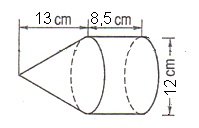
\includegraphics{bilder/zylinderkegel.png}
\end{aufgabe} 
\begin{aufgabe}\framebox{\qquad/5} ~ \\ 
Ein Ball aus Leder hat einen Durchmesser von $18\mathrm{\,cm}$. Berechne, wie viel Leder zur Herstellung des Balls ben\"otigt wird. (Reste und Verschnitt m\"ussen nicht beachtet werden.)
\end{aufgabe} 
\begin{center} \begin{framed} Erh\"ohtes Niveau (6 Punkte) \end{framed} \end{center}\begin{aufgabe}\framebox{\qquad/6} ~ \\ 
Eine Pyramide hat eine quadratische Grundfl\"ache mit der Seitenl\"ange $12\mathrm{\,cm}$  und eine H\"ohe von $12\mathrm{\,cm}$. Gesucht ist der Radius eines Kegels, der das gleiche Volumen und die gleiche H\"ohe hat.
\end{aufgabe} 
\end{flushleft} 
    \end{document}